\documentclass[tikz,border=12pt]{standalone}
\usepackage{amsmath}
\usepackage{amssymb}
\usepackage{tikz}

\definecolor{ink}{HTML}{0F172A}
\definecolor{linegray}{HTML}{64748B}
\definecolor{tokenfill}{HTML}{E2E8F0}
\definecolor{positionfill}{HTML}{F8FAFC}
\definecolor{resultfill}{HTML}{CBD5E1}

\begin{document}
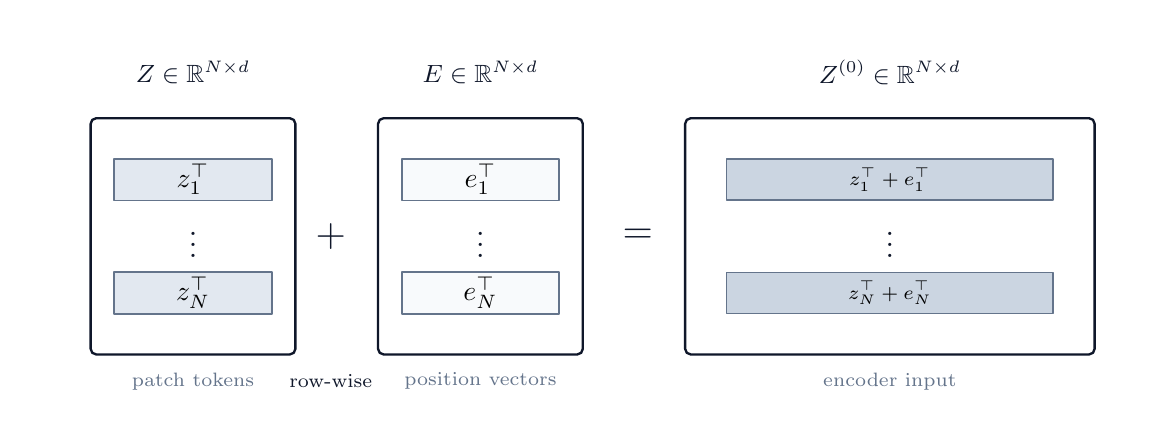
\begin{tikzpicture}[
  font=\sffamily,
  line cap=round,
  line join=round,
  row/.style={
    draw=linegray,
    line width=0.6pt,
    minimum height=0.52cm,
    inner sep=2pt,
    align=center
  },
  matrix box/.style={
    draw=ink,
    line width=0.85pt,
    rounded corners=2pt,
    inner sep=0pt
  }
]
  \fill[white] (-0.8,-0.75) rectangle (13.35,4.15);

  % Patch-token matrix.
  \node[ink, font=\small] at (1.3,3.58)
    {$Z \in \mathbb{R}^{N\times d}$};
  \draw[matrix box] (0,0) rectangle (2.6,3.0);
  \node[row, fill=tokenfill, minimum width=2.0cm] at (1.3,2.22)
    {$z_1^\top$};
  \node[ink, font=\large] at (1.3,1.5) {$\vdots$};
  \node[row, fill=tokenfill, minimum width=2.0cm] at (1.3,0.78)
    {$z_N^\top$};
  \node[linegray, font=\scriptsize] at (1.3,-0.34)
    {patch tokens};

  % Positional-embedding matrix.
  \node[ink, font=\small] at (4.95,3.58)
    {$E \in \mathbb{R}^{N\times d}$};
  \draw[matrix box] (3.65,0) rectangle (6.25,3.0);
  \node[row, fill=positionfill, minimum width=2.0cm] at (4.95,2.22)
    {$e_1^\top$};
  \node[ink, font=\large] at (4.95,1.5) {$\vdots$};
  \node[row, fill=positionfill, minimum width=2.0cm] at (4.95,0.78)
    {$e_N^\top$};
  \node[linegray, font=\scriptsize] at (4.95,-0.34)
    {position vectors};

  % Row-wise addition.
  \node[ink, font=\Large] at (3.05,1.5) {$+$};
  \node[ink, font=\scriptsize] at (3.05,-0.34)
    {row-wise};
  \node[ink, font=\Large] at (6.95,1.5) {$=$};

  % Encoder input after positional information is added.
  \node[ink, font=\small] at (10.15,3.58)
    {$Z^{(0)} \in \mathbb{R}^{N\times d}$};
  \draw[matrix box] (7.55,0) rectangle (12.75,3.0);
  \node[row, fill=resultfill, minimum width=4.15cm, font=\scriptsize]
    at (10.15,2.22) {$z_1^\top+e_1^\top$};
  \node[ink, font=\large] at (10.15,1.5) {$\vdots$};
  \node[row, fill=resultfill, minimum width=4.15cm, font=\scriptsize]
    at (10.15,0.78) {$z_N^\top+e_N^\top$};
  \node[linegray, font=\scriptsize] at (10.15,-0.34)
    {encoder input};
\end{tikzpicture}
\end{document}
